\section{Introduction}

The hardware nodes of a cloud service provider are often dedicated to running a
single cloud service component.
%todo: think about cite something, e.g., facebook citation, and figure out if
%they actually use dedicated nature to do both, in which case we can combine
%above and next sentance
One hopes that this dedicated nature (i.e. fixed role in the service using a
fixed software stack) can be exploited to obtain the required performance
(e.g., 99\% tail latency) while minimizing the energy used (and thus the cost
for providing the service). 
The importance of this task is magnified by the presence of increasingly
constrained energy budgets in data centers~\cite{SmoothOperator, Dynamo}. 
However, the performance and energy use of a system is an emergent property of
the myriad interactions between application software, operating systems,
hardware along with the offered load. 
%todo: above ends where, why is this a however?
%As OS developers do we really understand what is going on and the impact of
%each of our decisions?
Rather than focusing on the design and implementation
of  particular, local or global, mechanisms and policies for tuning performance
and energy consumption, perhaps we need a greater understanding of the
underlying impacts and dynamics of performance and energy consumption.   

When designing and implementing an operating system there is a dizzying array
of mechanisms and policies one must consider, both locally and globally, that
could impact individually and through their interaction  the performance and
energy use of the system; What should run after handling an interrupt, when
should interrupts be enabled and disabled, how should I/O bound and CPU bound
work be identified and prioritized,  when should the processors be put into
sleep states, what sleep state should be used, what values should processor
energy setting be set to, should setting be dynamically adjust and if so when
and why, what time constants should be used for various background tasks,
should device settings be used to adjust their interrupt behaviour, when and to
what degree should polling versus interrupt driven I/O be exploited and for
which devices or logical streams, what if any settings should be exposed for
manual adjustment or advice elicitation, should a cooperative, preemptive or
hybrid scheduling be used?  Each decision can have both expected and unexpected
impact on the realized performance and energy usage that will arise when the
system is put into production, running particular applications and offered
loads. 

Do the decisions we make in the design and implementation of the OS really have
a significant impact on tuning the performance and energy consumption for
network driven processing?  
%Do we understand the emergent interactions our software has with the hardware,
%application and the workload characteristics from this perspective?
For that matter what if any headroom exist to improve the performance and
energy consumption, for dedicated processing, or can we at best expect to only
trade one off for the other?   
We have experimentally explored these questions
and found the results fascinating, revealing both expected and unexpected
results.

\begin{wrapfigure}{r}{.6\columnwidth}
\vspace{-0.3in}
\begin{center}
%\hspace{-.22in}
 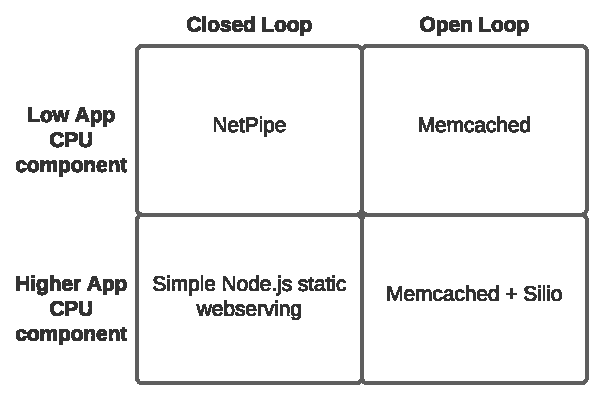
\includegraphics[width=.6\columnwidth]{figures/expgrid.pdf}
\vspace{-.5in}
%\caption{Setup}
        %\label{fig:setup}
%      \vspace{-.24in}
\end{center}    
\end{wrapfigure}  
In this paper we present findings from a detailed study of the emergent impact
that server operating systems design and implementation, and its interaction
with hardware settings, can have on the combination of performance and energy. 
We use four network driven workloads to explore a grid of open versus closed
loop dynamics along with lower and higher application CPU requirements. 
 We have run thousands of experiments capturing detailed time series log data
on every network interrupt.  This data includes, a high precision timestamp,
Joules consumed, instructions and cycles executed, sleep states entered, and
last level cache misses.  We exhaustively sweep three hardware settings; 1) NIC
Interrupt delay (ITR), 2) Dynamic Voltage and Frequency Scaling (DVFS) and 3)
Running Average Power Limit (RAPL) over both a general purpose OS (Linux) and
an application specific Library OS (libOS).    Figures 2-5 illustrates four
example landscapes we observed for selected workload configurations.  
 
\begin{figure*}[htb]
\centering	
\begin{minipage}[t]{0.45\textwidth}
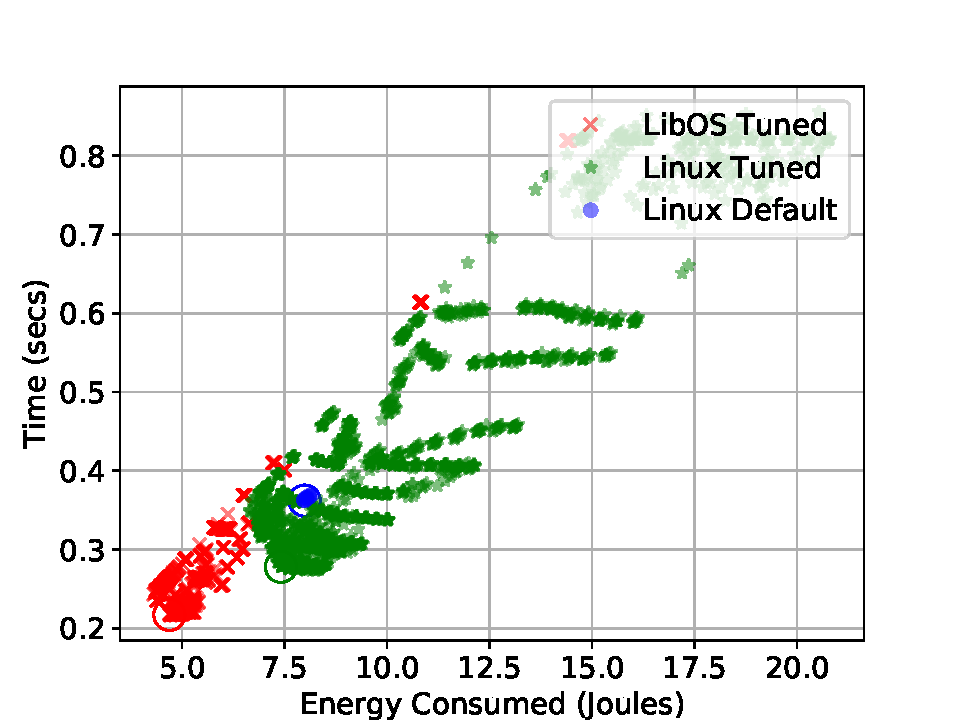
\includegraphics[width=\textwidth]{osdi_figures/netpipe_8192_overview.pdf}
	\caption{Netpipe 8KB overview}
	\label{fig:netpipe8Kov}
\end{minipage}
\begin{minipage}[t]{0.45\textwidth}
	\includegraphics[width=\columnwidth]{osdi_figures/mcd_600K_overview.pdf}
	\caption{Memcached 600K QPS}
	\label{fig:mcdov}
\end{minipage}
\begin{minipage}[t]{0.45\textwidth}
	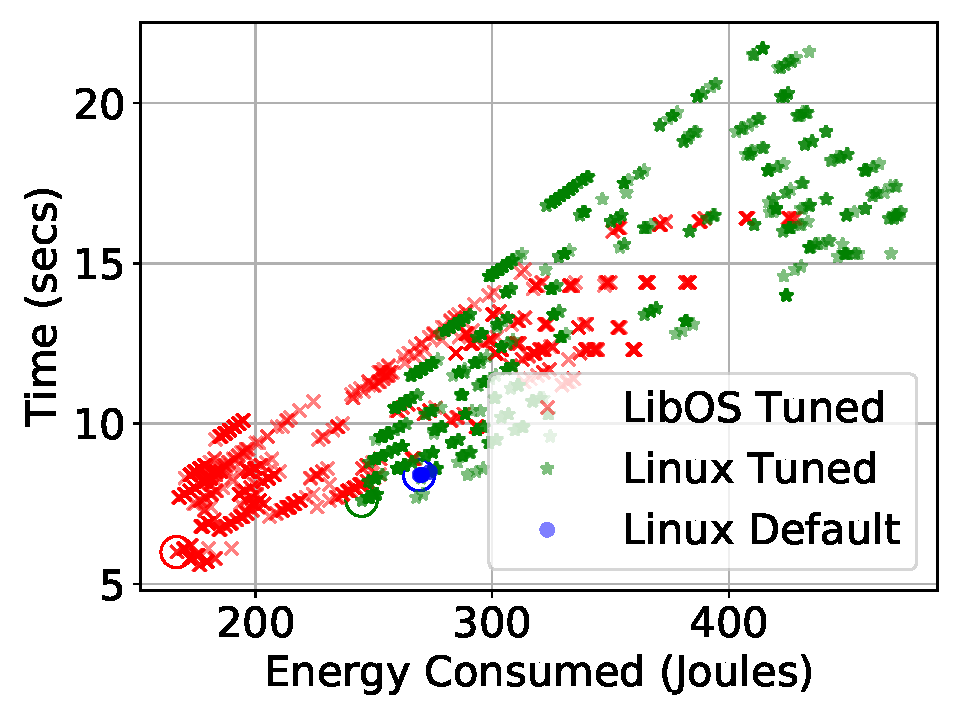
\includegraphics[width=\textwidth]{osdi_figures/nodejs_overview.pdf}
	\caption{NodeJS overview}
	\label{fig:nodejsov}
\end{minipage}
\begin{minipage}[t]{0.45\textwidth}
	\includegraphics[width=\columnwidth]{osdi_figures/mcdsilo_100K_overview.pdf}
	\caption{MemCached Silo 100K QPS}
	\label{fig:mcdsilioov}
\end{minipage}
\end{figure*}
Each point in these graphs represent the results of an experimental run.  Using
the log for each run we calculate the total energy consumed and a workload
specific measure.  In the case of netpipe and node.js this value is the time to
complete some fixed number of sequential transactions in a closed loop setting.
In the case of netpipe (figure~\ref{fig:netpipe8Kov}) the time is to complete
approximately two hundred thousand 8Kb message round trips with a client
configured with same OS and hardware setting as the server.  Whereas for
Node.JS (figure ~\ref{fig:nodejsov}) it is the time required to serve two
hundred thousand requests for a minimal static webpage driven by a client configured with default Linux software.  Whereas in the case of
Memcached and Memcached-Silo, open loop workloads, we use the reported 99\%
tail latency experienced while under a specific load of some number of queries
per second for a period of 20 seconds.  Specifically, for Memcached
(figure~\ref{fig:itr_figure}), the offered load is 600 queries per second
generated using the ETC Facebook benchmark.  For Memcached-Silo
(figure~\ref{fig:mcdsilioov}), the offered load is 200 queries per second.  In
both cases, for our hardware and Linux stack these offered load rates are close
too but does not exceed the systems capacity further we filter any results that
do not satisfy an SLA of 500 micro seconds.  

  Each experimental run uses a unique setting for the three hardware parameters we study,
(ITR, DVFS, and RAPL) for the two operating systems we consider.  We do not
modify the operating systems nor do we modify application software beyond in
choosing in Linux what is considered a production quality configuration.  Each
graph in some sense demonstrates the overall energy vs performance landscape
that can be achieved for the given workloads and the software bases considered.
Later sections of the paper present  details of how we conducted the
experiments
and  focus on results for “optimal” points in this landscape for both operating
systems.  They also identify the result obtained when running the experiment on
Linux using its defaults for these parameters.    The next section, however,
discusses the landscapes more broadly and summarizes the core finds
with respect to OS design and implementation.  

